\section{Experimental Evaluation}
\label{sec:experiments}

This this section we present our experimental evaluation of \VizRecDB.
We performed a detailed analysis of both execution engines of \VizRecDB\ with
respect to correctness and performance.
We used a suite of real and synthetic datasets listed in Table \ref{} to test the
performance of our techniques.
All experiments were run on a single
machine with XXX Intel Xeon E7 processors with 8 GB
RAM.

We begin with an evaluation of the DBMS-backed execution engine, followed by an
evaluation of our custom solution.

\subsection{DBMS-backed Execution Engine}
\label{sec:dbms_execution_engine}

As mentioned in Section \ref{}, our DBMS-based execution engine leverages the
DBMS API to execute queries corresponding to views using the existing DBMS
infrastructure.
While this approach has the advantage of agnostic of the underlying DBMS, its
limitations include lack of fine grained control over sharing of table scans and
lack of ability to prune low-utility views.

We ran all our experiments in this section on two database systems: a
row-oriented database (denoted as ROW in the following figures) and a
column-oriented database (COL).
The reason was evaluating both systems was that we expect certain
optimizations to work better for row-stores vs. column stores.
The main metric we are concerned with in this section is performance.
Since this version of the execution engine exhaustively explores all views and
then orders them by utility, we are guaranteed to get the top-$k$ views with
perfect accuracy.
All latency measurements were repeated three times and the results were
averaged.

We start with an evaluation of the basic framework and study the effect of
adding each individual optimization.\\

\noindent {\it Basic Framework}: The basic DBMS-backed execution engine
sequentially executes individual view queries for each possible view.
Figure \ref{fig:baseline_size} and Figure \ref{fig:baseline_views} show the
\VizRecDB\ latency when using the basic framework.
Figure \ref{fig:baseline_size} shows the change in latency with changes in table
size while Figure \ref{fig:baseline_views} shows the impact of view number on
the latency.
In Figure \ref{fig:baseline_size}, we fixed the number of views at 250 and
varied the number of rows from 100K to 1M, whereas in Figure
\ref{fig:baseline_views}, we fixed the number of rows at 1M and varied the
number of views from 50 - 250.
As expected, we see that the latency of the basic framework is directly
proportional to the number of rows as well as the number of views in the table.
We see that the column store runs wildly faster than the row store in each run.
This is expected because individual view queries only select one dimension
attribute and one measure attribute at a time, making each query in the column
store significantly faster than the same query in the row store which must load
all columns.

Finally, we note that the row and column store respectively take between 10-100s
and between 50-500s to evaluate all views.
These time scales are simply unacceptable for interactive applications, and
therefore, we must aggressively optimize our queries. \\

% \begin{figure}[h] 
% \centerline{
% \resizebox{4cm}{!} {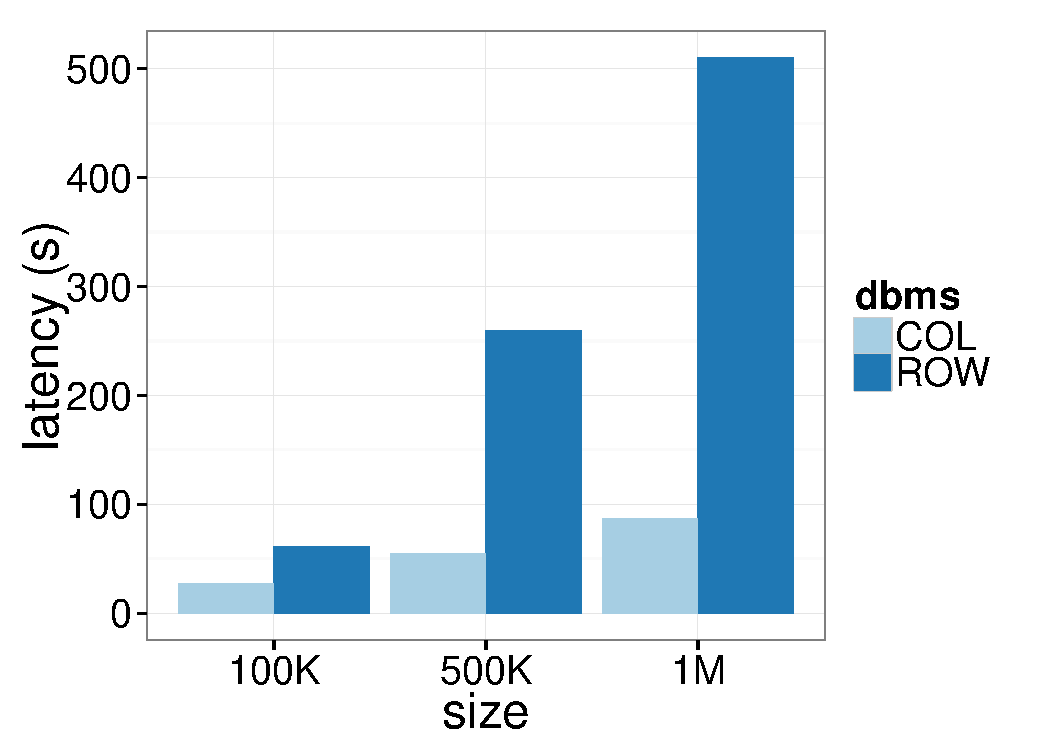
\includegraphics {Images/baselines_by_size.pdf}}
% \resizebox{4cm}{!} {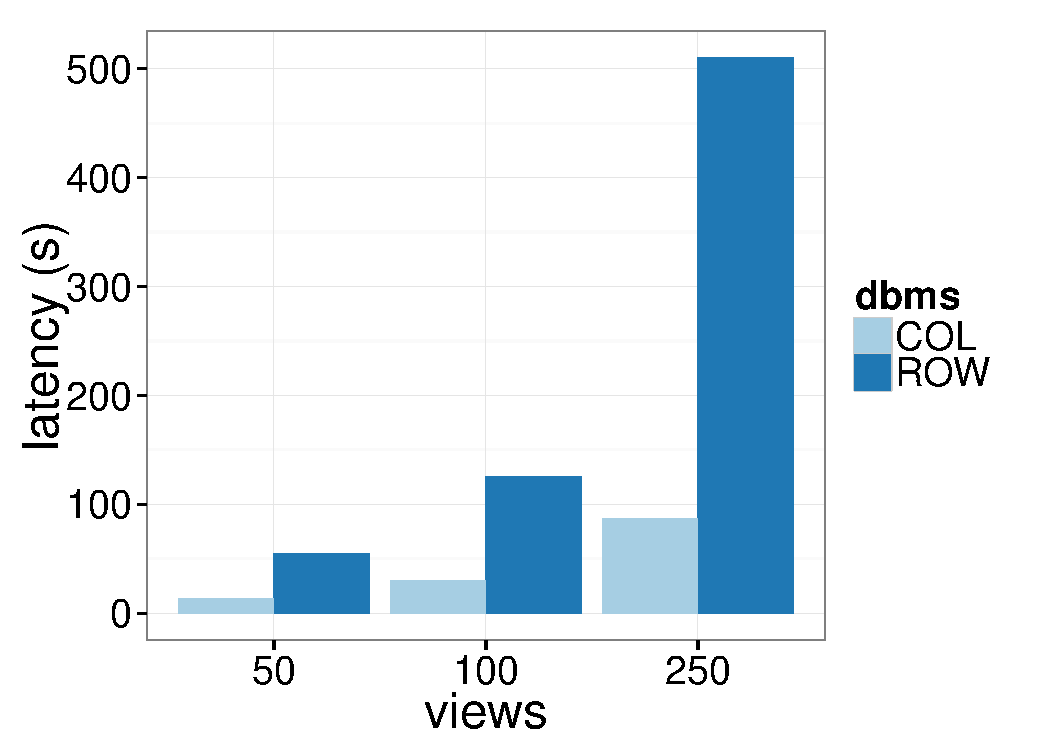
\includegraphics {Images/baselines_by_views.pdf}}
% }
% \end{figure}

\begin{figure}[h]
\centering
\begin{subfigure}{0.49\linewidth}
\centering
{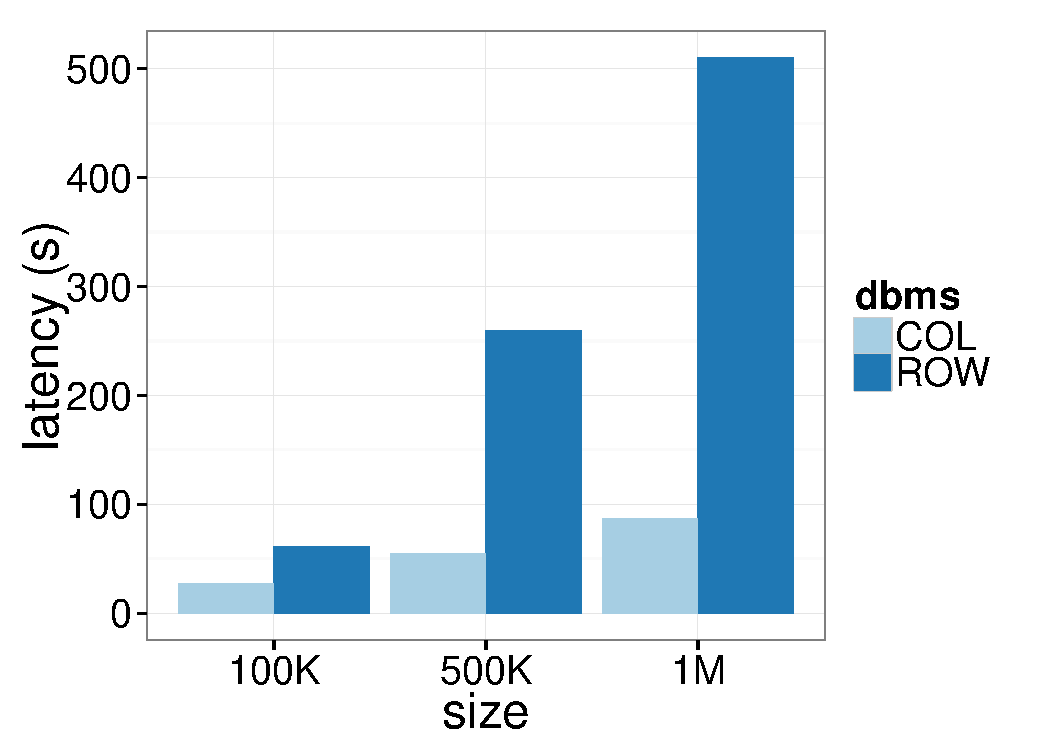
\includegraphics[width=4.2cm] {Images/baselines_by_size.pdf}}
\caption{Latency vs. Table size}
\label{fig:baseline_size}
\end{subfigure}
\begin{subfigure}{0.49\linewidth}
\centering
{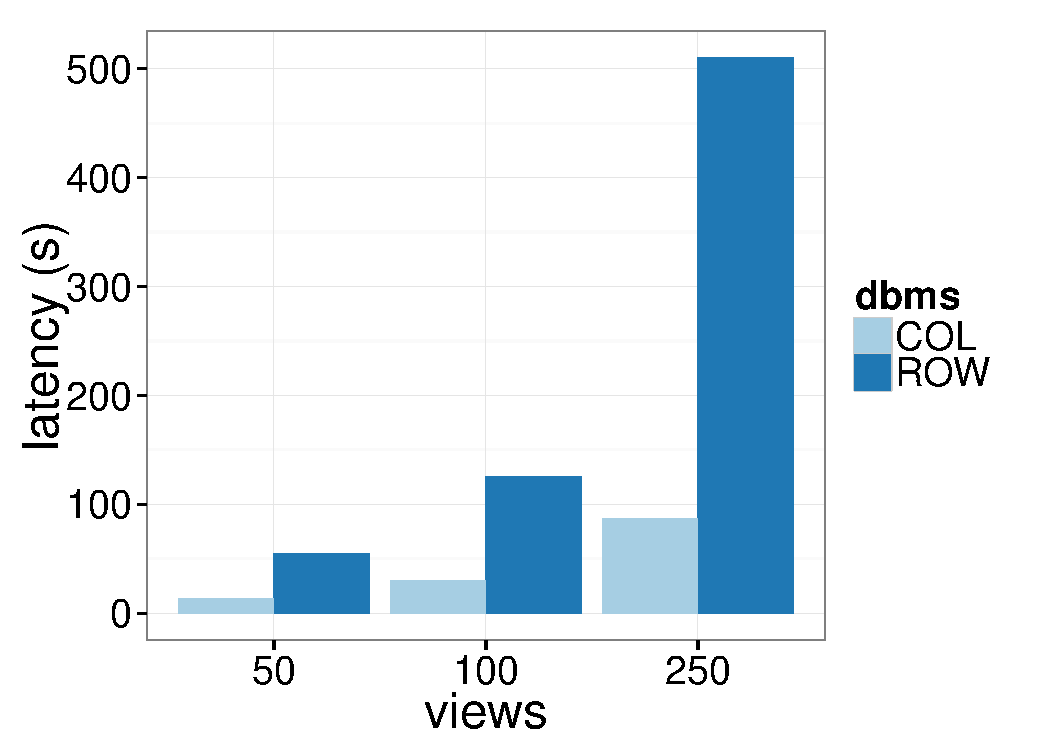
\includegraphics[width=4.2cm] {Images/baselines_by_views.pdf}}
\caption{Latency vs. Num Views}
\label{fig:baseline_views}
\end{subfigure}
\label{fig:baselines}
\caption{Latency of Basic Framework}
\end{figure}

\noindent {\it Combining Multiple Aggregates}: Next, we study the impact of
combining multiple aggregates within the same query.
The goal of this optimization is to evaluate multiple views at once by keeping
track of multiple aggregates for the same dimension attribute.
For a synthetic dataset of 1M rows and 1000 views (50 dimension and 20 measure
attributes), we varied the number of aggregations performed per query
($n_{agg}$) between 1 and 20 and measured the impact on latency.
As shown in Figure \ref{fig:multi_agg}, latency reduces as we increase the
number of aggregations performed per query.
This optimization shows promise both in the row store as well as the column
store, athough we note that the optimization has diminishing returns as more
state must be stored and, in the case of the column store, more columns must be
read. \\

\begin{figure}[h]
\centering
{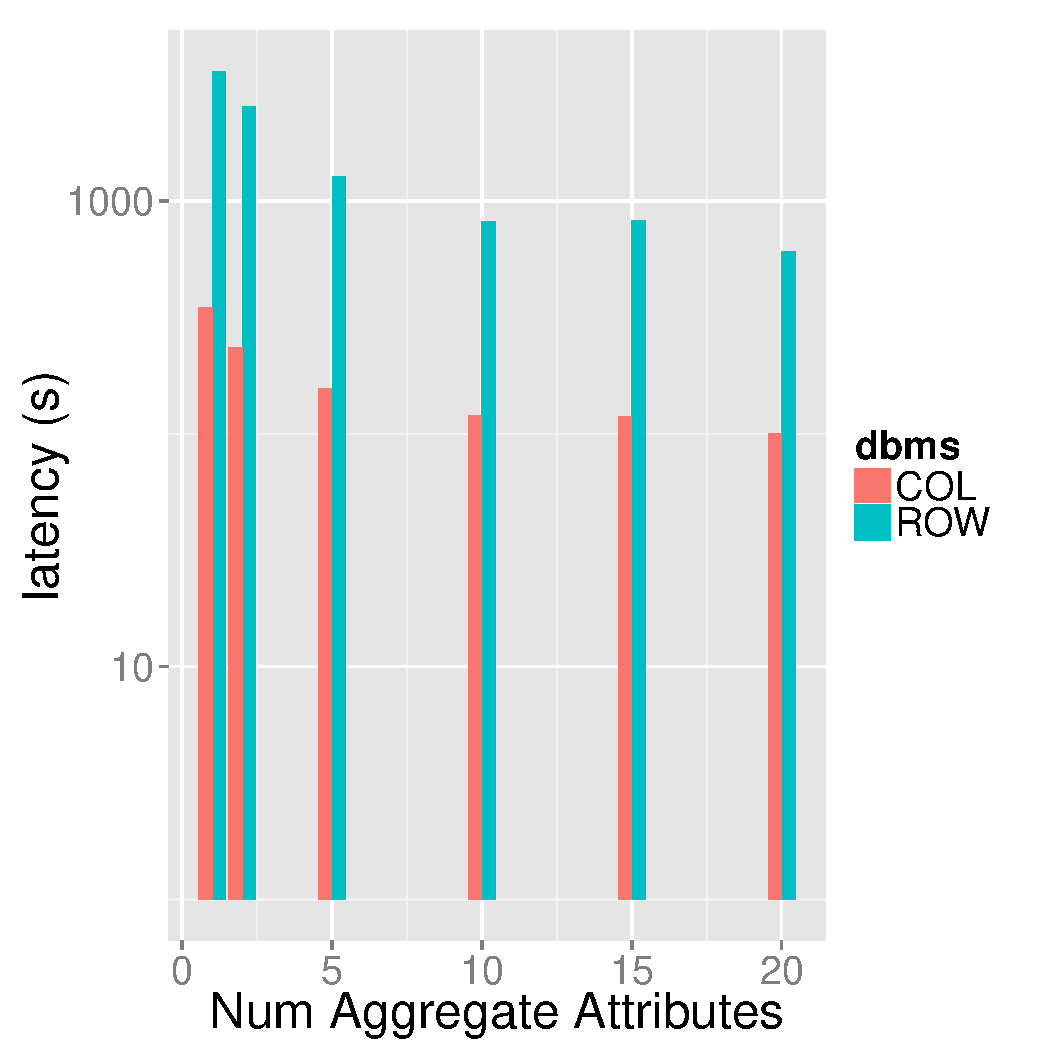
\includegraphics[width=6cm] {Images/multi_agg.pdf}}
\caption{Latency vs. number of aggregates}
\label{fig:multi_agg}
\end{figure} 

\noindent {\it Combining Multiple Group Bys}: In this set of experiments, we
study the effect of combining multiple group by attributes into one query.
Section \ref{} briefly discussed how the impact of this optimization was not
clear since it increases the total number of groups significantly and therefore
leads to higher cost of processing intermediate results.

To evaluate this optimization, we generated a synthetic dataset with 1M rows, 1
measure attribute and 20 dimension attributes such that each dimension attribute
was independently generated and had exactly 10 distinct values.
Since each dimension attribute is independent of the others and has 10 distinct
values, the total number of distinct groups produced when we construct a query
with $p$ group-by attributes is $10^p$.

We ran \VizRecDB\ on this dataset and varied the number of group-by
attributes in view queries ($n_{gb}$) between 1 and 20.
Figure \ref{fig:multi_gb_same} shows the results for this experiment.
We see that for the row-store, the best latency is obtained for number of
groups=$10^4$.
Beyond $10^5$, the performance degrades drastically. 
For the column-store, we see a relatively small improvement in latency
for $10^2$, however, once again, after $10^5$, the performance becomes
much worse.
The reason for this is as follows: as we combine group by attributes, the number
of distinct groups increases exponentially ($10^{n_{gb}}$). 
As a result, the memory required for the grouping (hash-based or sort based)
also increases significantly.
Once this memory requirement hits the pre-configured upper limit (e.g. say the
memorycap in the column store or working memory in the row store), the
performance degrades significantly.

\begin{figure}[h]
\centering
\begin{subfigure}{0.49\linewidth}
\centering
{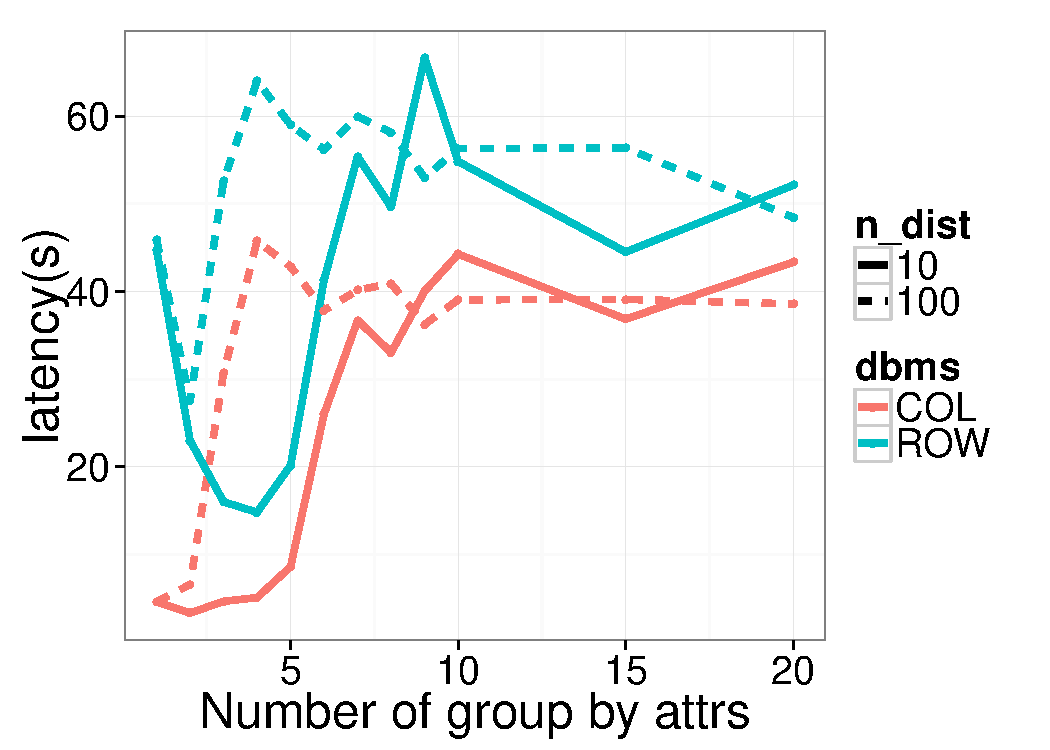
\includegraphics[width=4.2cm] {Images/multi_gb_same.pdf}}
\caption{Latency vs. Num of Groups}
\label{fig:multi_gb_same}
\end{subfigure}
\begin{subfigure}{0.49\linewidth}
\centering
{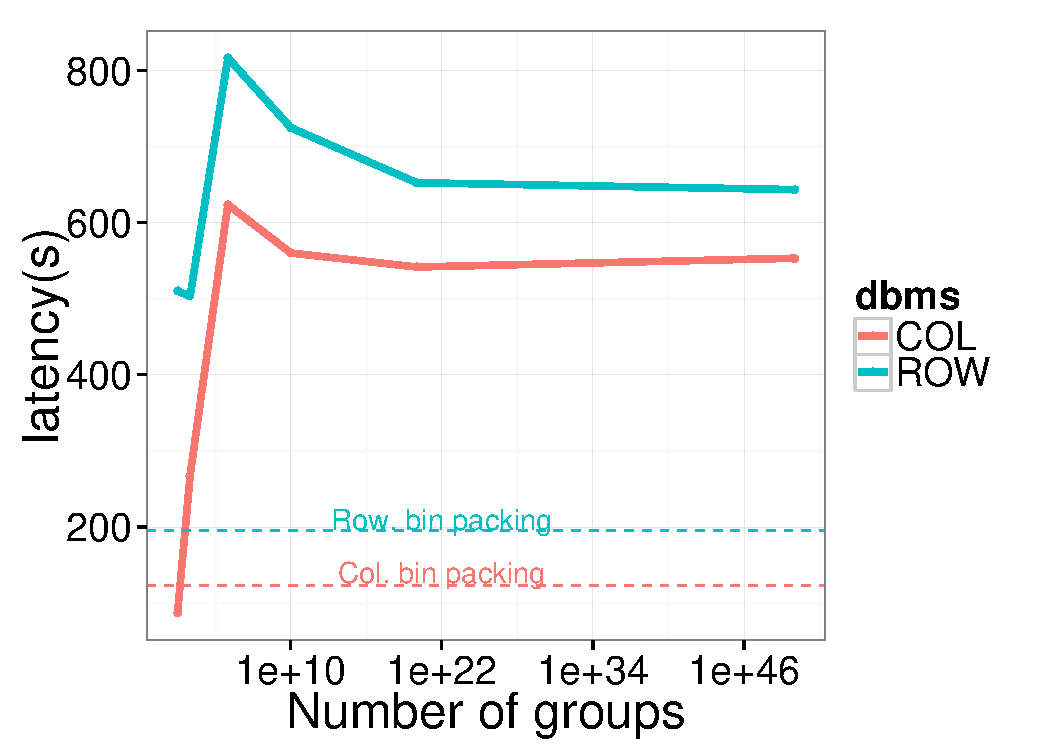
\includegraphics[width=4.2cm] {Images/multi_gb.pdf}}
\caption{Latency vs. Num Dimensions}
\label{fig:multi_gb_bp}
\end{subfigure}
\label{fig:multi_gb}
\caption{Effect of combining multiple groups}
\end{figure}

We can guard against the above performance degradation by ensuring that the
number of distinct groups never goes beyond a pre-configured upper limit.
From Figure \ref{fig:multi_gb_same}, we see that this limit is approximately
$10^5$ for both the row and column store.
Since we now have an upperlimit on the number of distinct groups, we can apply
the bin packing heuristic discussed in Section \ref{} to optimally group the
attributes. 
The heuristic ensures that the number of distinct groups produced by any
query is less than $10^5$. 
Figure \ref{fig:multi_gb_bp} shows the results of combining group-by attributes
for the synthetic dataset SYN1 with  1M rows, 50 dimension, 5 measures and with varying
number of distinct values in each dimension attribute. 
% There are two opposing forces at work here: increasing the number of dimensions
% in a query increases the execution time for that query, however, it reduces the
% number of queries that must be executed and hence reduces execution time.
We see trends similar to those in Figure \ref{fig:multi_gb_same}.
The horizontal lines denote the performance of the bin-packing heuristic that
optimally groups dimension attributes keep the number of groups below the
upper limit.
We see that the heuristic performs significantly better for the row-store but
slightly worse for the column store.\\

\noindent {\it Parallel Query Execution}: 
Executing view queries in parallel can provide significant performance gains;
however, a high degree of parallelism can lead to a performance drop off for
several reasons. Potential reasons include disk contention, RAM usage, lock
contention, context switches and cache line contention \cite{Postgres_wiki}. 

\begin{figure}[h]
\centering
{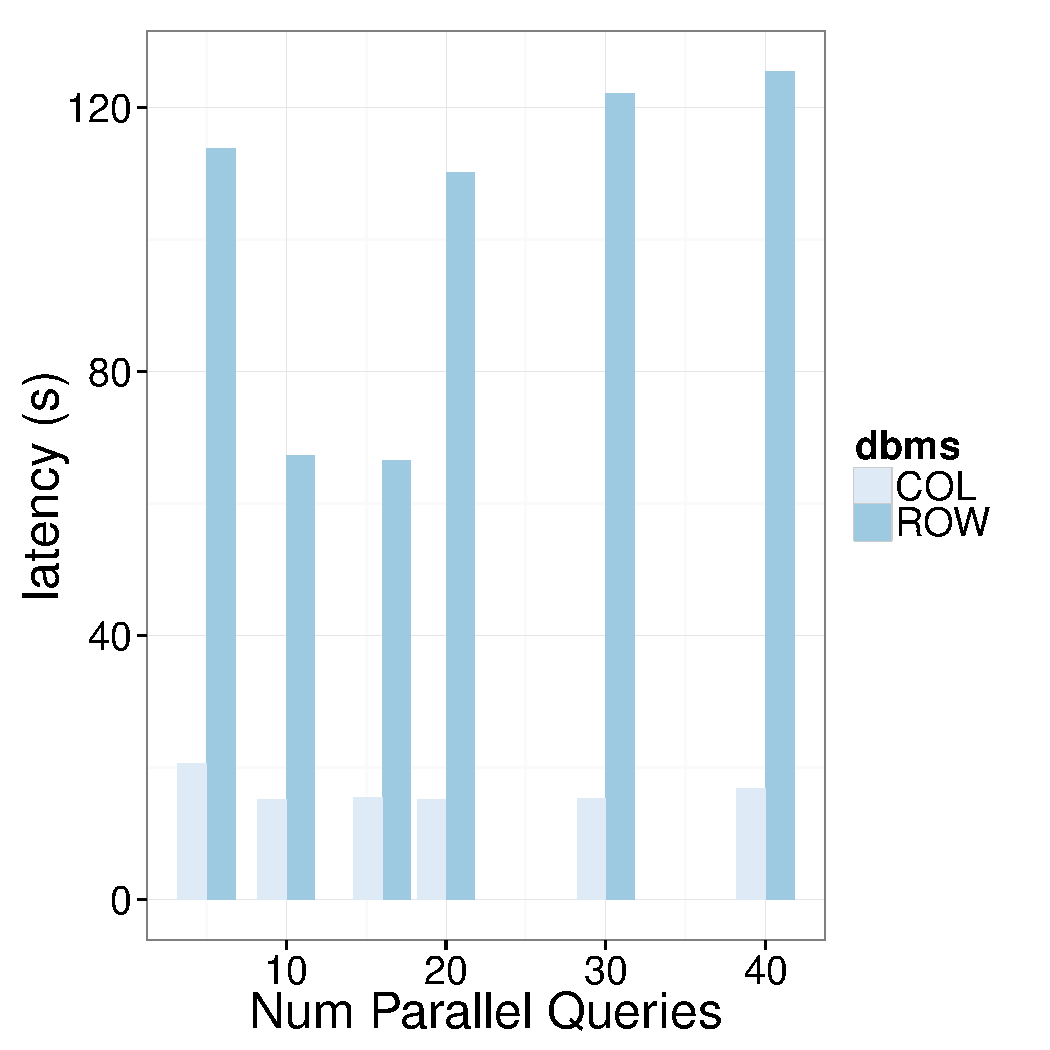
\includegraphics[width=6cm] {Images/parallel_noop.pdf}}
\caption{Effect of parallelism}
\label{fig:parallelism}
\end{figure} 

Figure \ref{fig:parallelism} illustrates this issue: we varied the number of
queries running in parallel on the DBMS and measured the latency of our system.
As expected, low levels of parallelism produce performance gains but high
parallelism leads to degraded performance.
For our system, the optimal number of queries to run in parallel is
approximately $16$ (equal to the number of cores).
For other systems, we recommend users that they set the number of parallel
queries to the maximum number of parallel queries that can be run in
their DBMS without performance degradation.
If this number is not easily available, a simple experiment as shown in Figure
\ref{fig:parallelism} can help approximate the right amount of parallelism. 

\noindent {\it Combining Target and Comparison Views}:
The last optimization we evaluate is that of combining the target and comparison
views and running a single SQL query per view as opposed to two.
We expected this optimization to roughly halve the latency since each query
takes one table scan instead of two.\\

\noindent {\it All optimizations}:
Now that we have explored all our optimizations in detail, we pick the optimal
parameters discovered above and combine our optimizations to get the maximum
performance gain.
Figure \ref{} shows the latency of \VizRecDB\ when all optimizations have been
applied.
As we can see, we obtain a XXX speedup for the row store and a YYY speed up for
the column store.
Our optimizations have reduced the basic framework latency from 100s of seconds
to tens of seconds.

As we can see from the experiments above, aggressive optimization of queries can
give us speedups of several orders of magnitude.
However, as discussed before, the DBMS-backed engine suffers from the
limitations of the DBMS API and therefore cannot prune low-utility views.
In the next section, we evaluate our custom execution engine and each of its
heuristics to see how much speedup can be obtained by using these heuristics.

\subsection{Custom Execution Engine}
\label{sec:custom_execution_engine}

As discussed in Section \ref{}, we built a custom execution engine for
\VizRecDB\ to take advantage of sharing table scans and using intermediate
results to prune low-utility views.

In this section, we evaluate the various pruning heuristics developed for our
custom execution engine.
Our goal is to determine how effective our strategies are for pruning
low-utility views and their effect on \VizRecDB\ latency.
For each of our experiments, we measure three metrics: latency, accuracy and
utility distance.
As before, latency is the time taken by \VizRecDB\ to return the top-$k$ views.
Accuracy is the number of views that are present
both in the true top-$k$ views and the top-$k$ views returned by our algorithm.
Finally, utility distance is the difference between the average utility of
actual top-$k$ views and the average utility of the top-$k$ views generated by our algorithm.
Since the accuracy and utility distance of our heuristic depends on the
underlying data distribution, each run was repeated 20 times with the data
randomized between each run. We report the average over 20 runs. 
Note that we cannot directly compare the latency
of our custom execution engine to the latency of the DBMS-backed execution engine.
This is for multiple reasons including the fact that the custom engine must read
data from a disk file and convert data to main memory format on the fly and that
our implementation is in Java and not as optimized as a commercial DBMS.
Our goal is to highlight the relative performance benefits that can be obtained
by performing pruning.

Since the performance of pruning strategies is necessarily dependent on the
distribution of values in the underlying table, we evaluate our strategies on
real-world datasets.
These are shown in Table \ref{}.
For each dataset, we evaluate 4 strategies: 
(a) No Pruning (NO\_PRU): we make a
single pass of the data and keep running estimates of the utility. Once we have
seen all the data, we return the top-$k$ views; 
(b) Hoeffding Intervals (HOEFF): pruning based on Hoeffding intervals (Section
\ref{});
(c) 95\% Confidence Intervals (95\_CI): pruning based on 95\% confidence
intervals (Section \ref{}); and 
(d) Multi-armed Bandit (MAB): pruning based on the multi-armed bandit
formulation (Section \ref{}).
For each of our datasets, we varied $k$, the number of views to choose, between
1 and 25 (a realistic upper limit on the number of views presented to the user)
and measured the latency, accuracy and utility distance for each of our
heuristics.

Let is first examine the accuracy and utility distance for our heuristics. \\

\noindent {\it Accuracy and Utility Distance}:
Figure \ref{fig:bank_accuracy} to \ref{fig:dia_accuracy} show the impact of
heuristics on the accuracy of our results.
We examine the banking dataset first.
The true distribution of utilities for all views of the banking dataset is
shown in Figure \ref{fig:bank_utility_distribution}. 
In this chart, a vertical line corresponds to the $k$-th highest utility for
$k$=\{1\ldots10,15,20,25\}.
The highest utility corresponds to the right-most line while the 25-th highest
utility corresponds to the left-most line.
From the chart we see that the highest and second highest utility are spread
well apart from the rest of the utility; then the top 3-9th utilities are rather
similar, the 10th highest utility is separated from neighboring utilities by a
large value and then the remaining utilities are again close together.
We see that the impact of this utility distribution in the accuracy chart in
Figure \ref{fig:bank_accuracy}.
We find that the average accuracy of all three heuristics is pretty good for
$k$=1 and 2.
However, between $k$=3\ldots9, the accuracy suffers (consequence of similar
utility values).
After $k$=10, the performance of all our heuristics improves once again.

Now, let us examine how ``bad'' are our errors in finding the top-$k$.
We do so by looking at the utility distance (i.e. the average distance between
the average utility of the real top-$k$ views and the average utility of the
top-$k$ views picked by our heuristics).
Figure \ref{fig:bank_utility_dist} shows the utility distance for all of our
heuristics.
Note that NO\_PRU necessarily has 0 utility distance. 
We notice however, that all of our heuristics have 0 or almost 0 utility
distance.
That is, even when or top-$k$ heuristic picks a few incorrect views, the
selected views have utility very close to the real top-$k$ views.
This implies that even if our top-$k$ views are approximate, they are of high
value.
Another way to analyze mistakes in the top-$k$ views is by examining if the an
incorrectly returned view for the top-$k$ views also appears in the top-$2k$,
top-$3k$ or top-$4k$.
Figure \ref{} shows the results for the banking dataset.
We see that XXX,

\begin{figure}[h]
\centering
\begin{subfigure}{0.49\linewidth}
\centering
{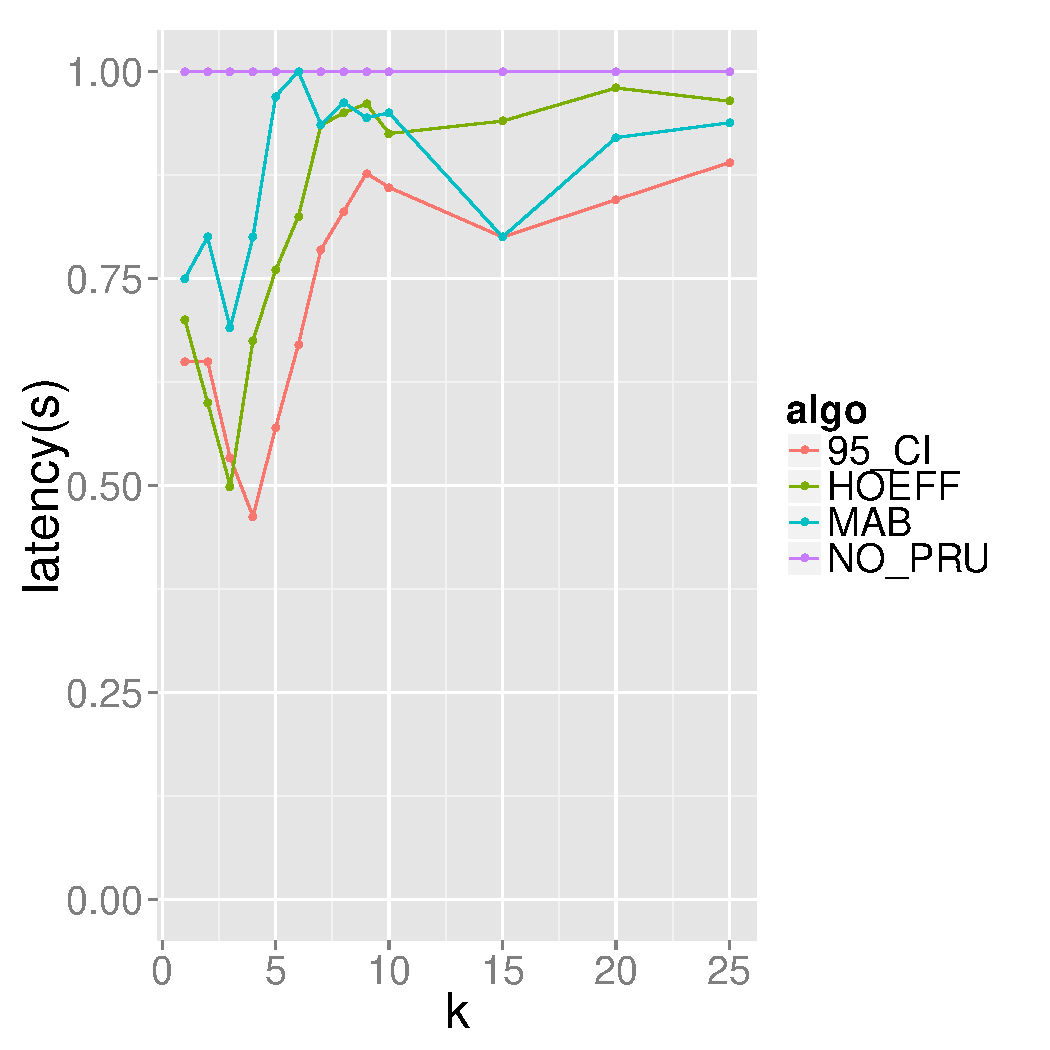
\includegraphics[width=4.2cm] {Images/bank_in_memory_accuracy.pdf}}
\caption{Accuracy of heuristic for bank dataset}
\label{fig:bank_accuracy}
\end{subfigure}
\begin{subfigure}{0.49\linewidth}
\centering
{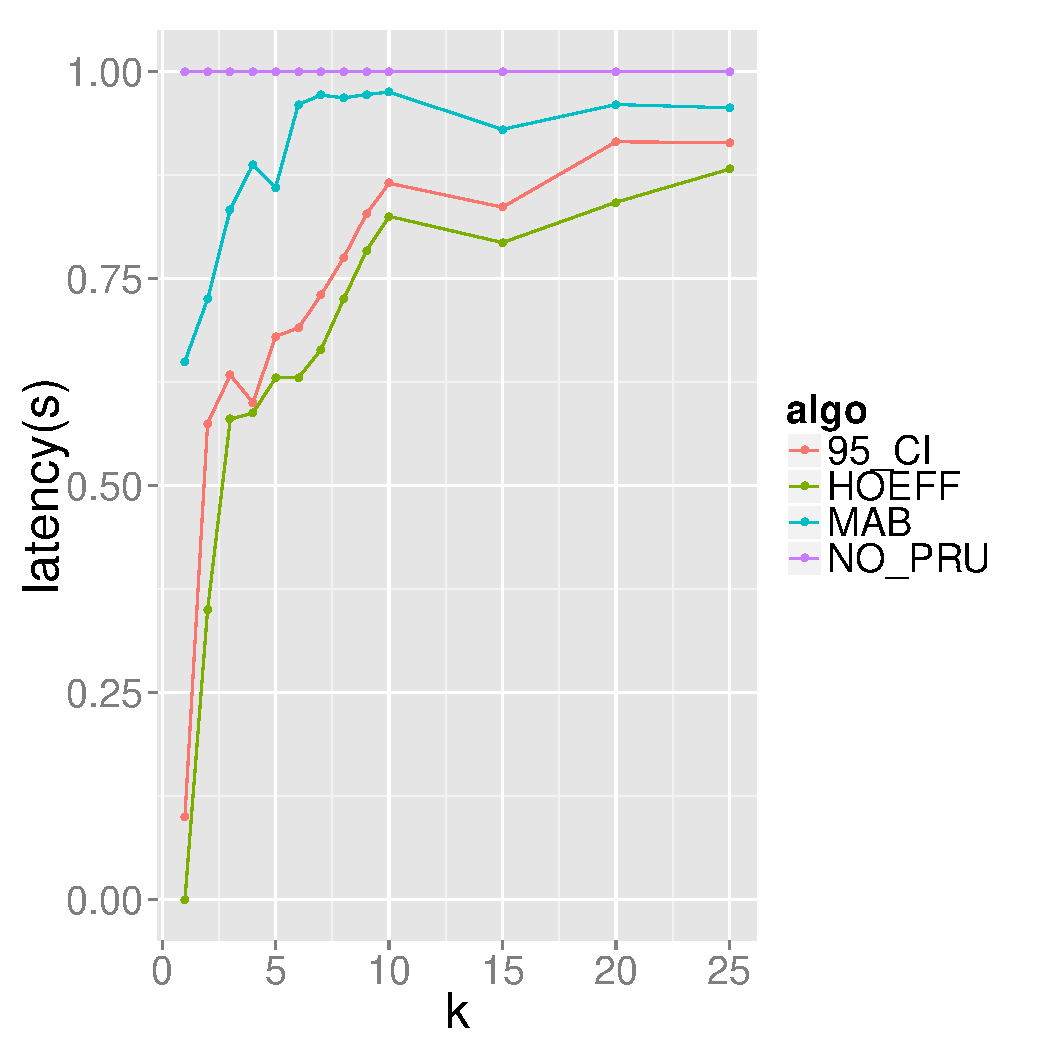
\includegraphics[width=4.2cm] {Images/dia_in_memory_accuracy.pdf}}
\caption{Accuracy of heuristics for diabetes dataset}
\label{fig:dia_accuracy}
\end{subfigure}
\label{fig:accuracy}
\caption{Accuracy of Heuristics}
\end{figure}


\begin{figure}[h]
\centering
\begin{subfigure}{0.49\linewidth}
\centering
{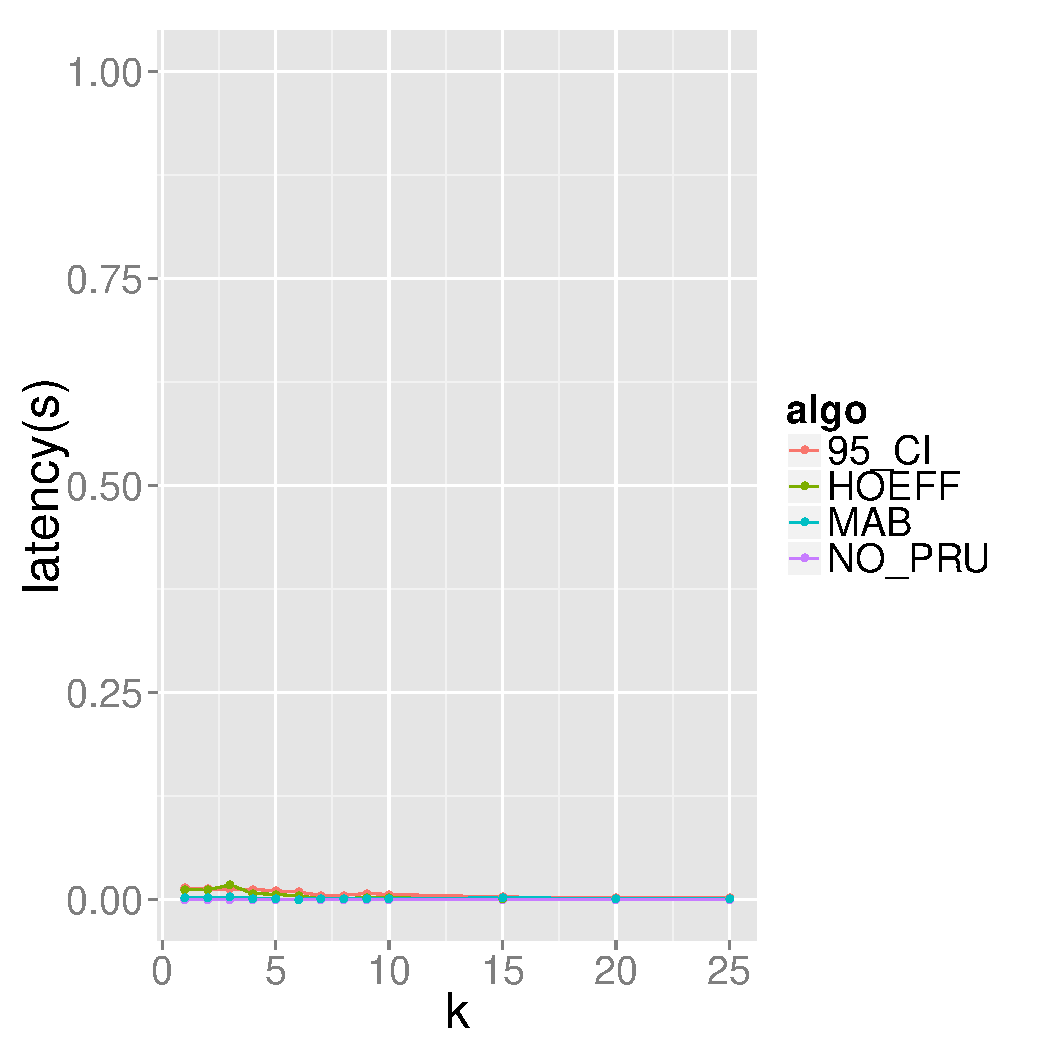
\includegraphics[width=4.2cm] {Images/bank_in_memory_utility_dist.pdf}}
\caption{Utility Distance of heuristic for bank dataset}
\label{fig:bank_utility_dist}
\end{subfigure}
\begin{subfigure}{0.49\linewidth}
\centering
{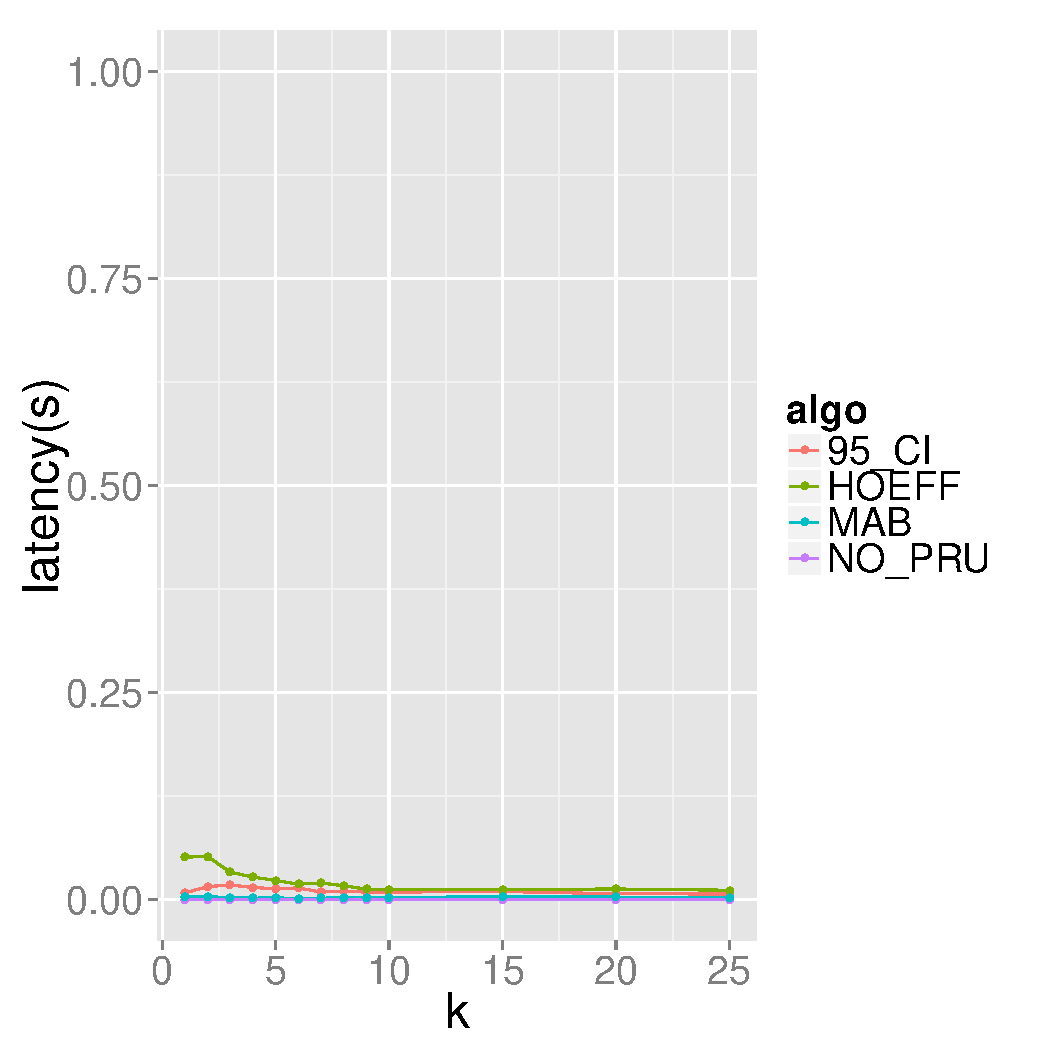
\includegraphics[width=4.2cm] {Images/dia_in_memory_utility_dist.pdf}}
\caption{Utility Distance of heuristics for diabetes dataset}
\label{fig:dia_utility_dist}
\end{subfigure}
\label{fig:accuracy}
\caption{Utility Distance for Heuristics}
\end{figure}

\begin{figure}[h]
\centering
{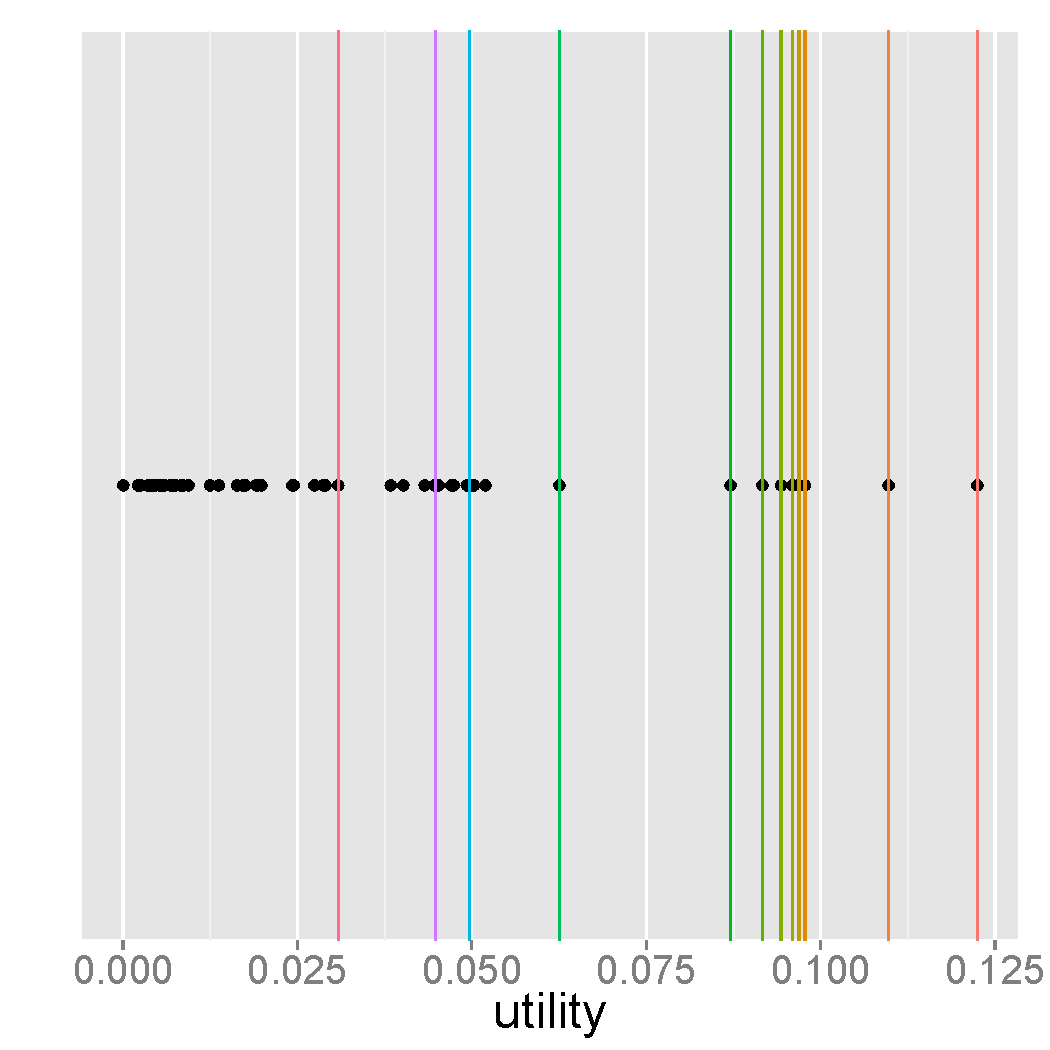
\includegraphics[trim = 0mm 50mm 0mm 50mm, clip, width=6cm]
{Images/bank_utility_distribution.pdf}}
\caption{Bank dataset: utility distribution}
\label{fig:bank_utility_distribution}
\end{figure}
\begin{figure}[h]
\centering
{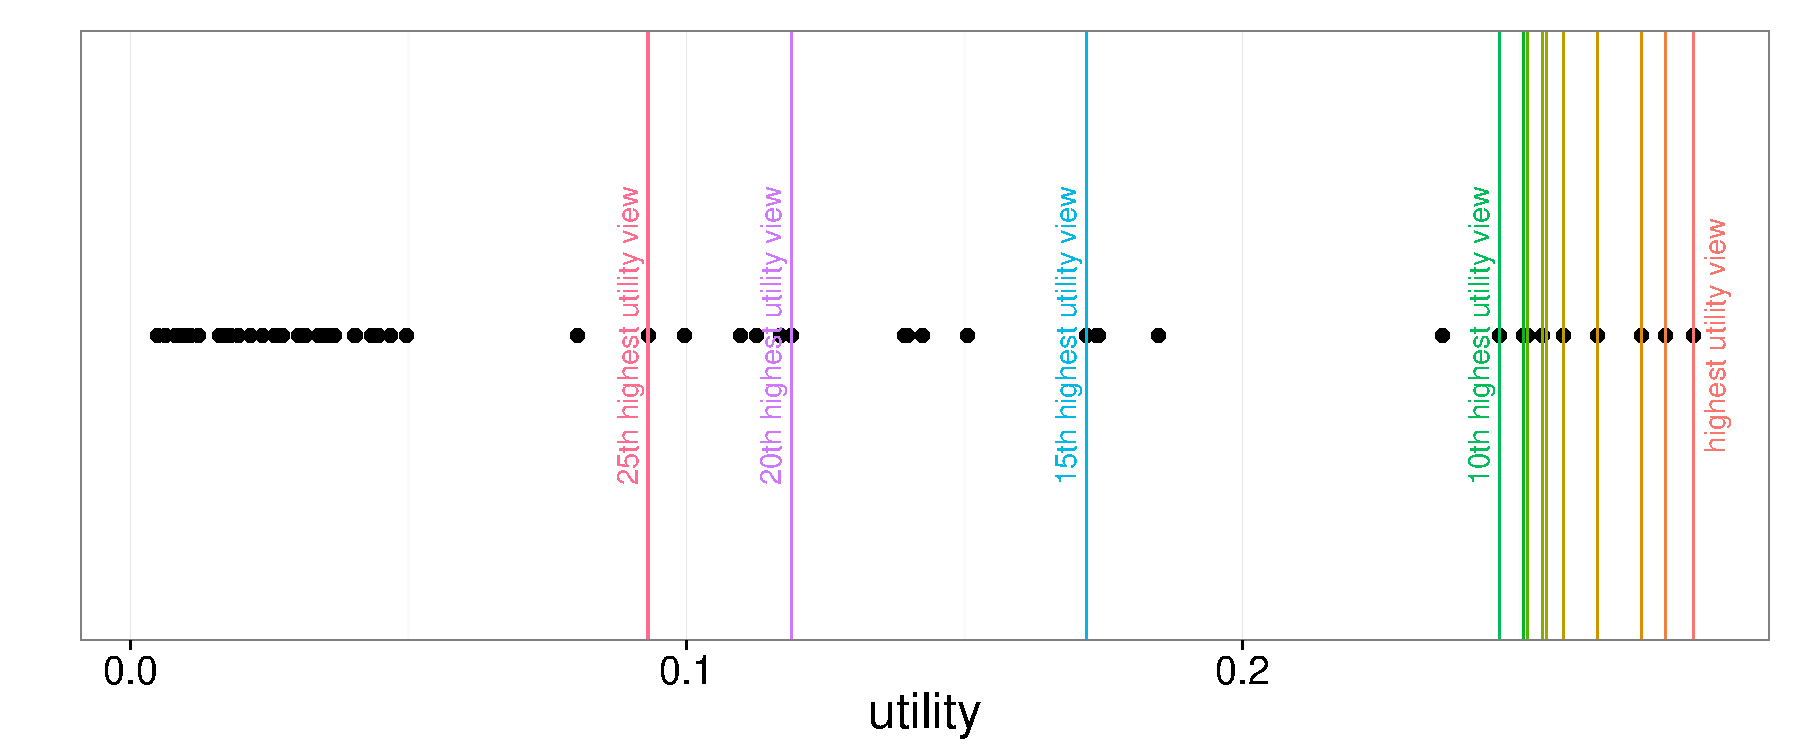
\includegraphics[trim = 0mm 50mm 0mm 50mm, clip, width=6cm]
{Images/diabetes_utility_distribution.pdf}}
\caption{Diabetes dataset: utility distribution}
\label{fig:diabetes_utility_distribution}
\end{figure}
 
Next, let us examine the results for the diabetes dataset.
The distribution of true utilities for all views in this dataset are shown in
Figure \ref{fig:diabetes_utility_distribution}.
Compared to the bank dataset, we see that the utilities for the diabetes are
very closely clustered from the top 1\ldots10 views. 
As a result, we expect more incorrectly chosen views in this range of $k$s.
Compared to that, the utilities around $k$=15, 20 and 25 are relatively widlely
spaced and we expect better accuracy for those $k$s.

% 95\_CI does the best among all our heuristics for the whole range of $k$ values.
% MAB and HOEFF produce similar accuracy values with MAB being slightly better
% than HOEFF.
% There are a few reasons why 95\_CI performs better: the MAB heuristic is tied to
% either accepting or discarding a view at the end of each phase; therefore, even
% if MAB is not very confidence in the action of accepting or discarding, it must
% reduce one view in each phase. HOEFF on the other hand is less accurate because
% XXX.
% All our heuristics however seem to have low accuracy for $k<10$. 

Now that we have characterized the accuracy of our techniques, we now turn to
latency.

\noindent {\it Latency}:
Next, let us look at how long it takes for our pruning strategies to work.
Figures \ref{fig:bank_latency} and \ref{fig:diabetes_latency} show the latency
of our heuristics for the banking and diabetes dataset.
The two charts look quite similar.
First off, we observe that the use of any of our heuristics reduces the latency
by at least 50\%.
For NO\_PRU and 95\_CI, for small $k$'s, we obtain a 90\% reduction in
latency. However, some of this reduction in latency is obtained at the cost
lower accuracy.
We observe that the latency of our HOEFF and 95\_CI increases almost linearly
with $k$.
Roughly speaking, this trend arises because we throw out fewer views as $k$
increases, so we must perform more computation for each record.
This trend is not seen in MAB because MAB's pruning of views is agnostic to
the number of views that must be selected.

In general, we see that it is possible to reduce latency by 50\% just by using
any of our heuristics.
If we want to achieve further performance gains, we must be willing to
tradeoff some accuracy.
The next set of experiments vary the parameters for each heuristic to study
the accuracy vs. latency tradeoff.\\

\begin{figure}[h]
\centering
\begin{subfigure}{0.49\linewidth}
\centering
{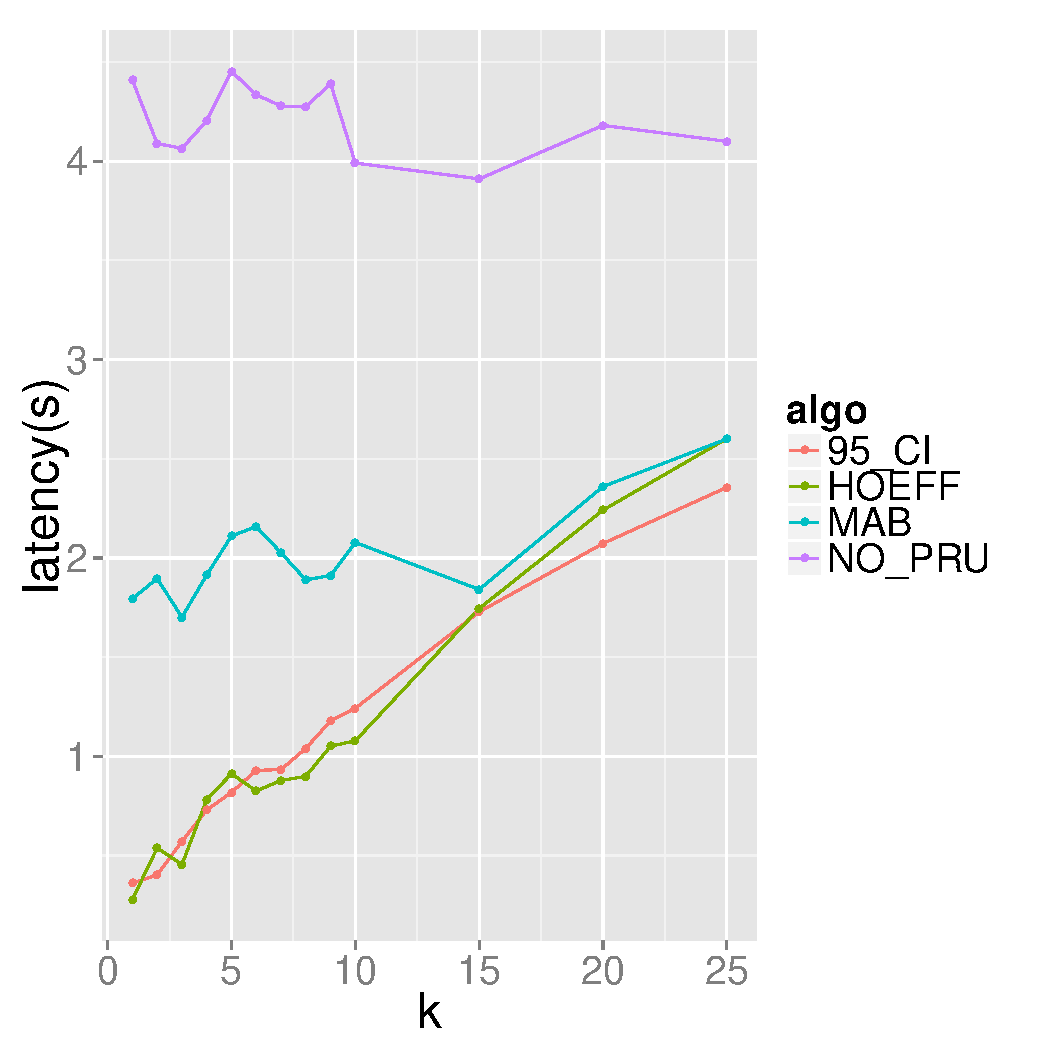
\includegraphics[width=4.2cm] {Images/bank_in_memory_latency.pdf}}
\caption{Bank dataset: latency}
\label{fig:bank_latency}
\end{subfigure}
\begin{subfigure}{0.49\linewidth}
\centering
{\includegraphics[width=4.2cm] {Images/diabetes_in_memory_latency.pdf.pdf}}
\caption{Diabetes dataset: latency}
\label{fig:diabetes_latency}
\end{subfigure}
\label{fig:accuracy}
\caption{Latency for Heuristics}
\end{figure}

\noindent {\it Accuracy vs. Latency}:
Our MAB and 95\_CI heuristics both have ``knobs'' we can use to study the
tradeoff between accuracy and latency.
In MAB, for example, we can tune the number of phases involved in
processing the entire file. 
Since MAB reduces the number of views by 1 after each phase, the number of
phases is directly proportional to the pruning power of our algorithm.
 a larger
number of phases means that MAB will throw away more views and sooner than expected.
While this will lead to lower latency, it will also lead to lower accuracy.
Figure \ref{} shows how latency and accuracy both reduce as we increase the
number of phases in MAB.
For 95\_CI, we can vary the $z$-score used as the
multiplier for our confidence interval. That is, we can decide to take a 50\% confidence interval, 80\%, 90\%
etc.
If we take a smaller confidence interval, we will have higher pruning and
therefore lower latency.
However, it will also lead to lower accuracy since we prune views with
lower confidence.
Figure \ref{} shows that as the $z$-score of the confidence interval increases,
the accuracy of our heuristics increases, but so does its latency.




